\begin{figure}[!htbp]
	\centering
	\begin{subfigure}[b]{0.7\textwidth}
		\centering
		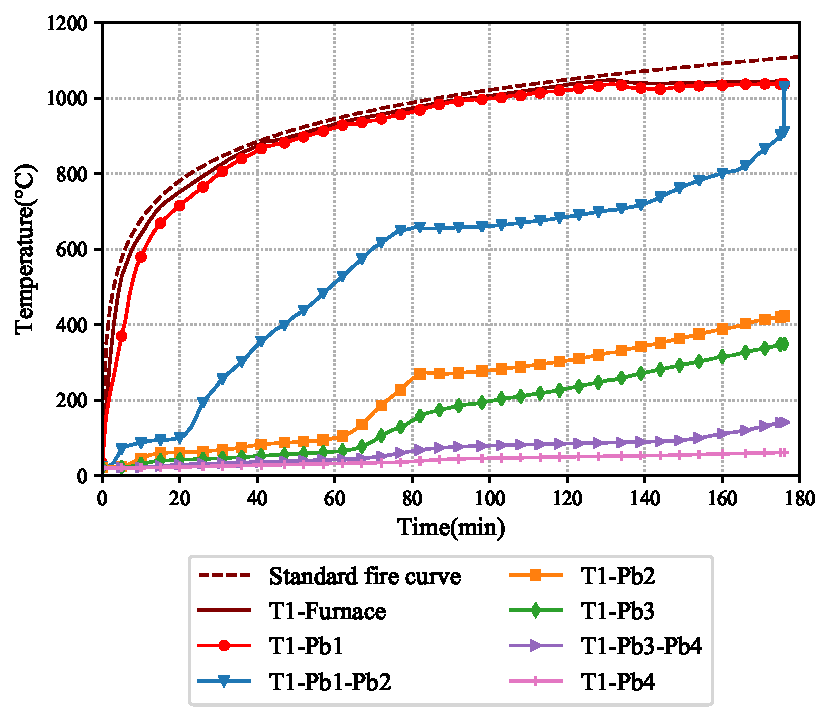
\includegraphics[width=\textwidth]{T1-Plasterboard.pdf}
		\caption{}
		\label{subfig:T1-Plasterboard}
	\end{subfigure}
	\begin{subfigure}[b]{0.7\textwidth}
		\centering
		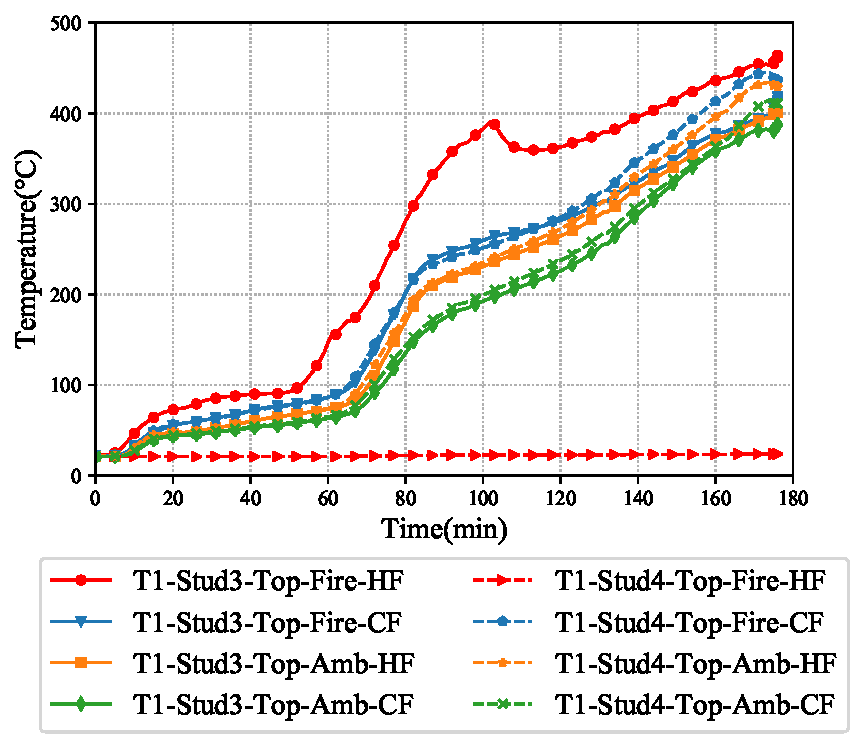
\includegraphics[width=\textwidth]{T1-Stud3-4-Top.pdf}
		\caption{}
		\label{subfig:T1-Stud3-4-Top}
	\end{subfigure}
	   \caption{Plasterboard and stud time-temperature curves of Test-T1 (a) Average plasterboard temperatures (b) Stud3 and 4 temperatures}
	   \label{fig:T1-PB-Stud}
	   \fontsize{10}{1}\textit{Note:Thermocouple T1-Stud4-Top-Fire-HF malfunctioned.}
\end{figure}

\begin{figure}[!htbp]
	\centering
	\begin{subfigure}[b]{0.7\textwidth}
		\centering
		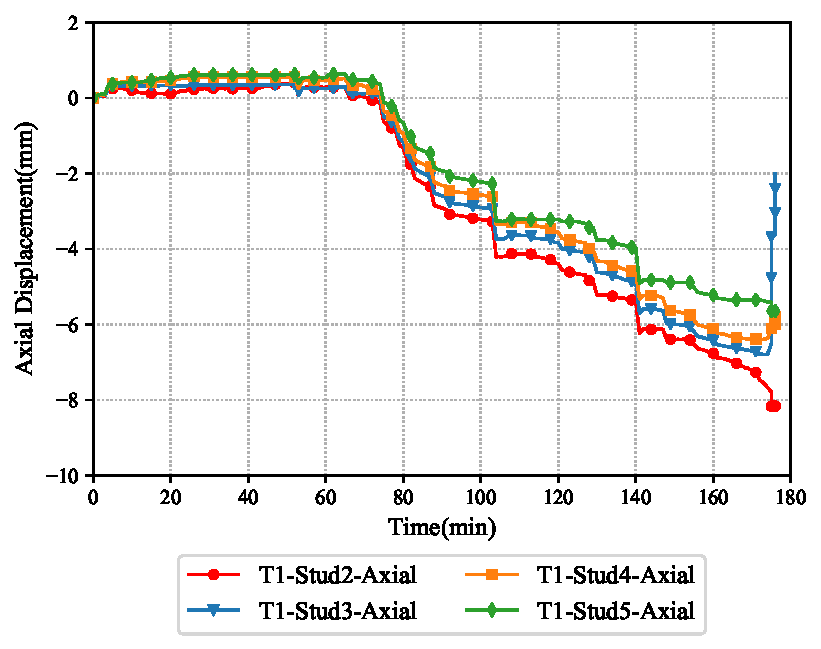
\includegraphics[width=\textwidth]{T1-Axial.pdf}
		\caption{}
		\label{subfig:T1-Axial}
	\end{subfigure}
	\begin{subfigure}[b]{0.7\textwidth}
		\centering
		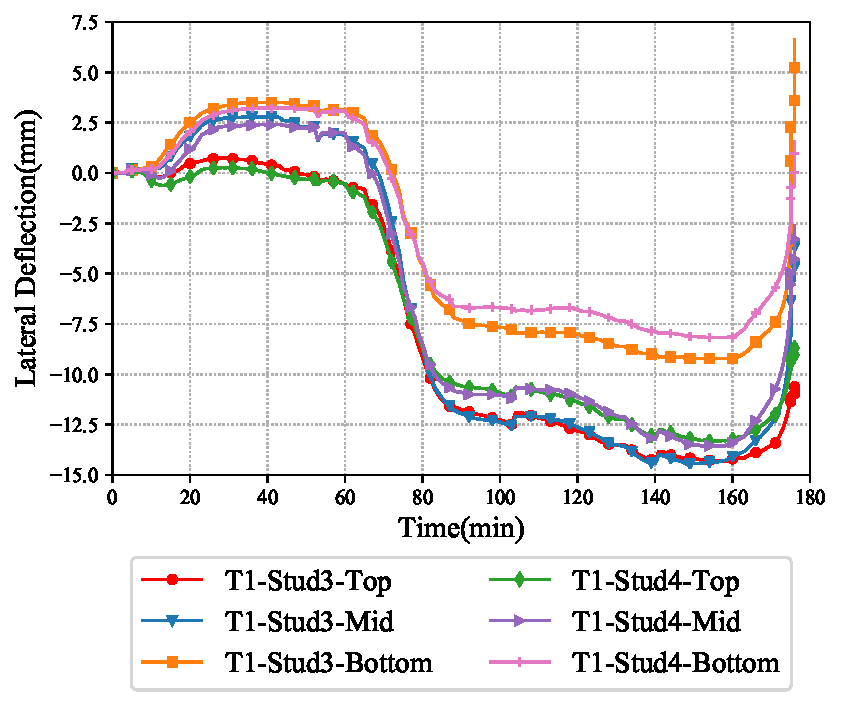
\includegraphics[width=\textwidth]{T1-Lateral.pdf}
		\caption{}
		\label{subfig:T1-Lateral}
	\end{subfigure}
	   \caption{Axial displacement and lateral deflection curves from Test-T1 (a) Axial displacement versus time (b) Lateral deflection versus time curves}
	   \label{fig:T1-Axial-Lateral}
\end{figure}

\begin{figure}[!htbp]
	\centering
	\begin{subfigure}[b]{0.3\textwidth}
		\centering
		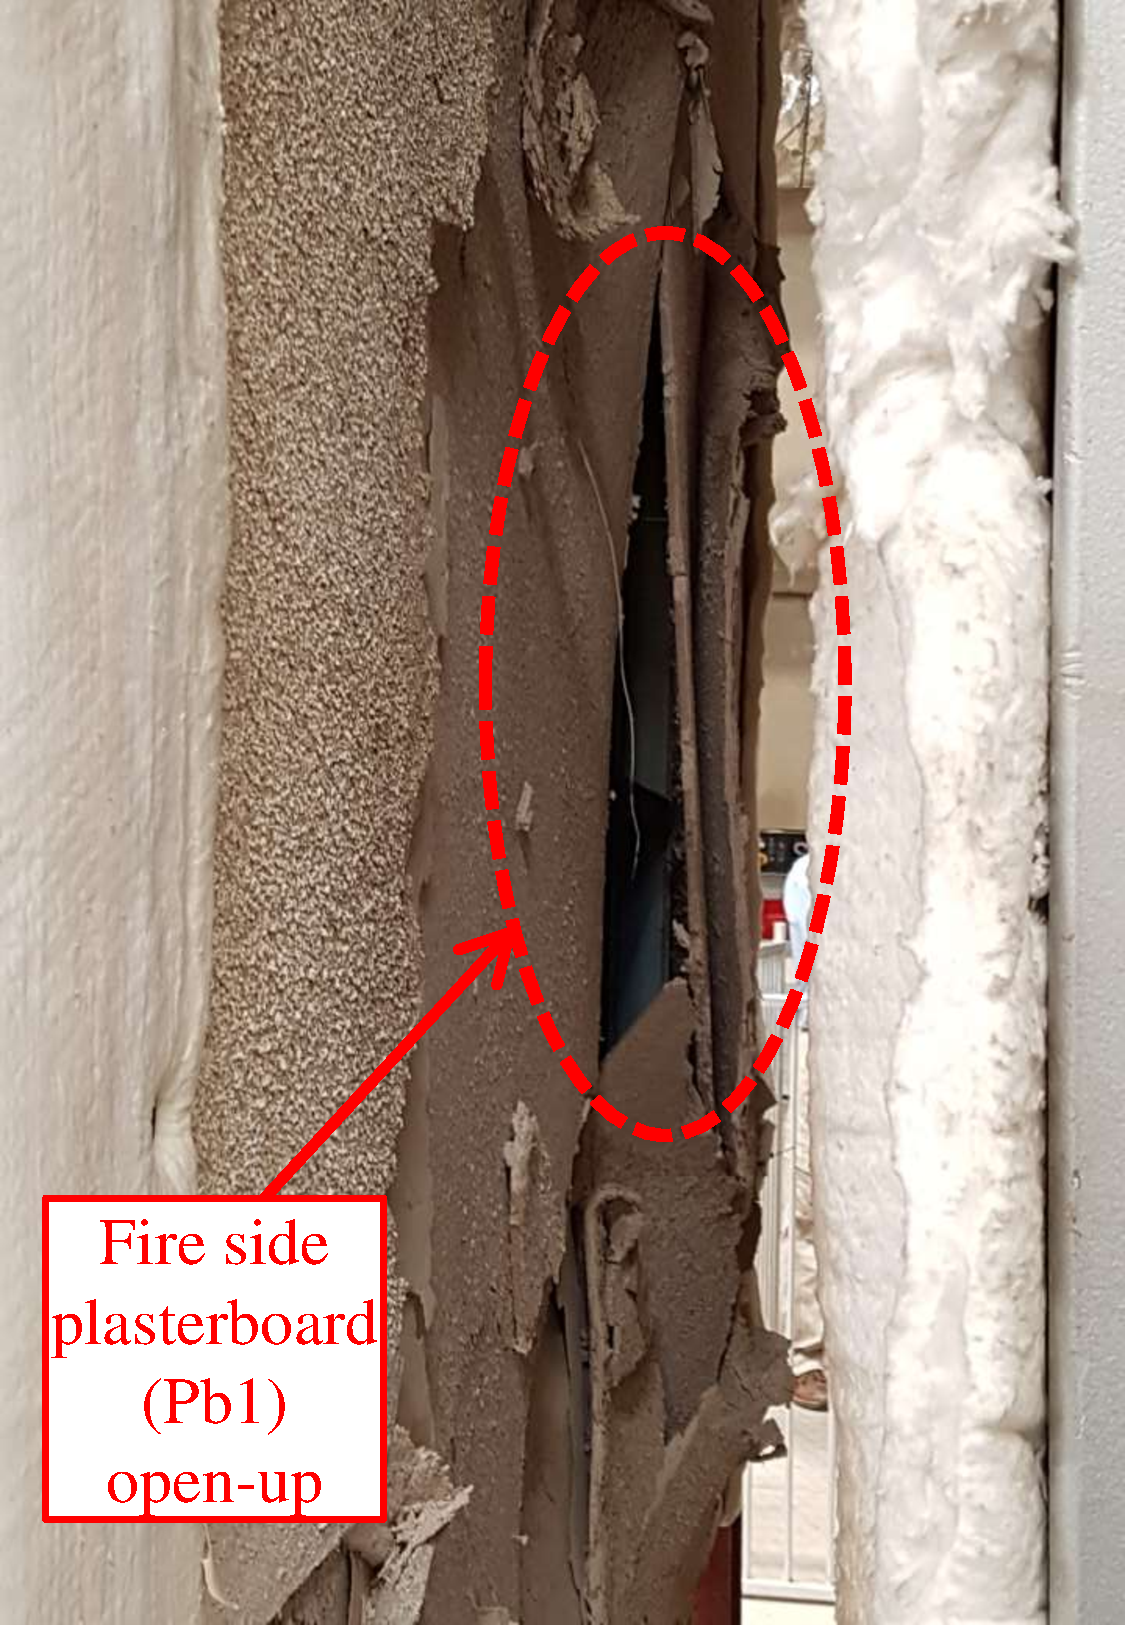
\includegraphics[width=\textwidth]{T1-fireside.pdf}
		\caption{}
		\label{subfig:T1-fireside}
	\end{subfigure}
	\begin{subfigure}[b]{0.3\textwidth}
		\centering
		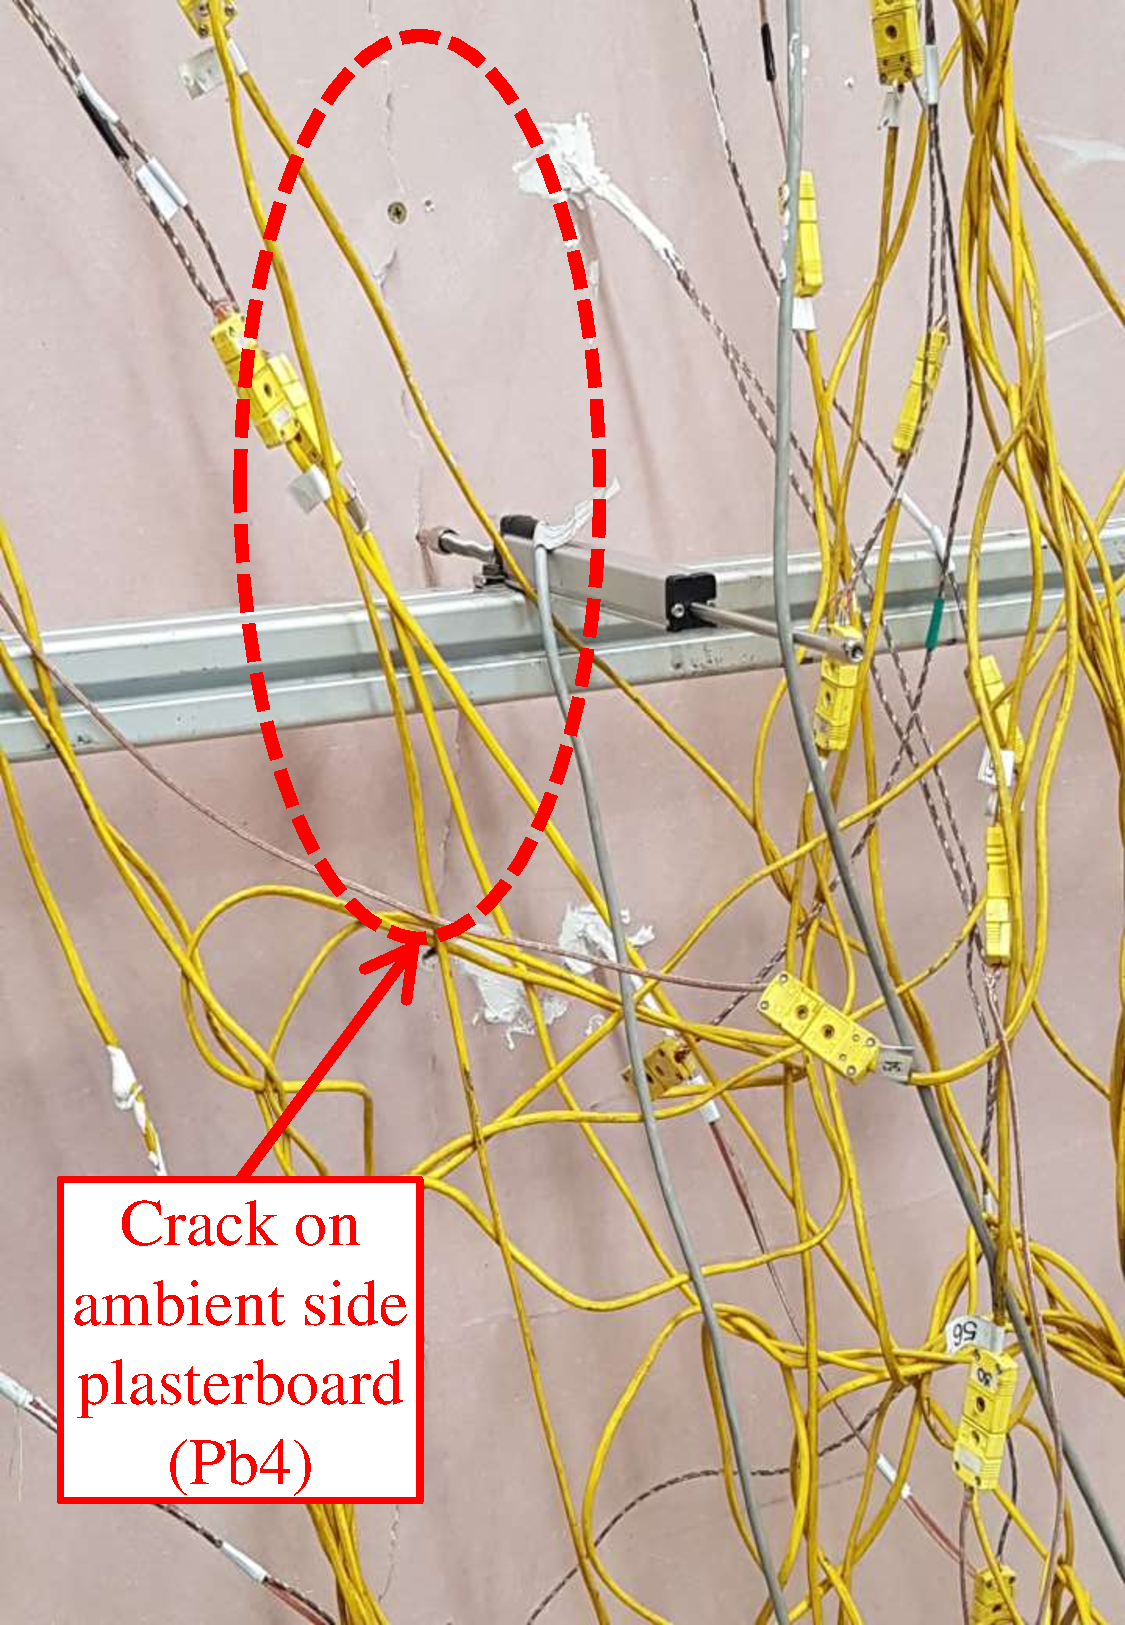
\includegraphics[width=\textwidth]{T1-ambientside.pdf}
		\caption{}
		\label{subfig:T1-ambientside}
	\end{subfigure}
	\begin{subfigure}[b]{0.3\textwidth}
		\centering
		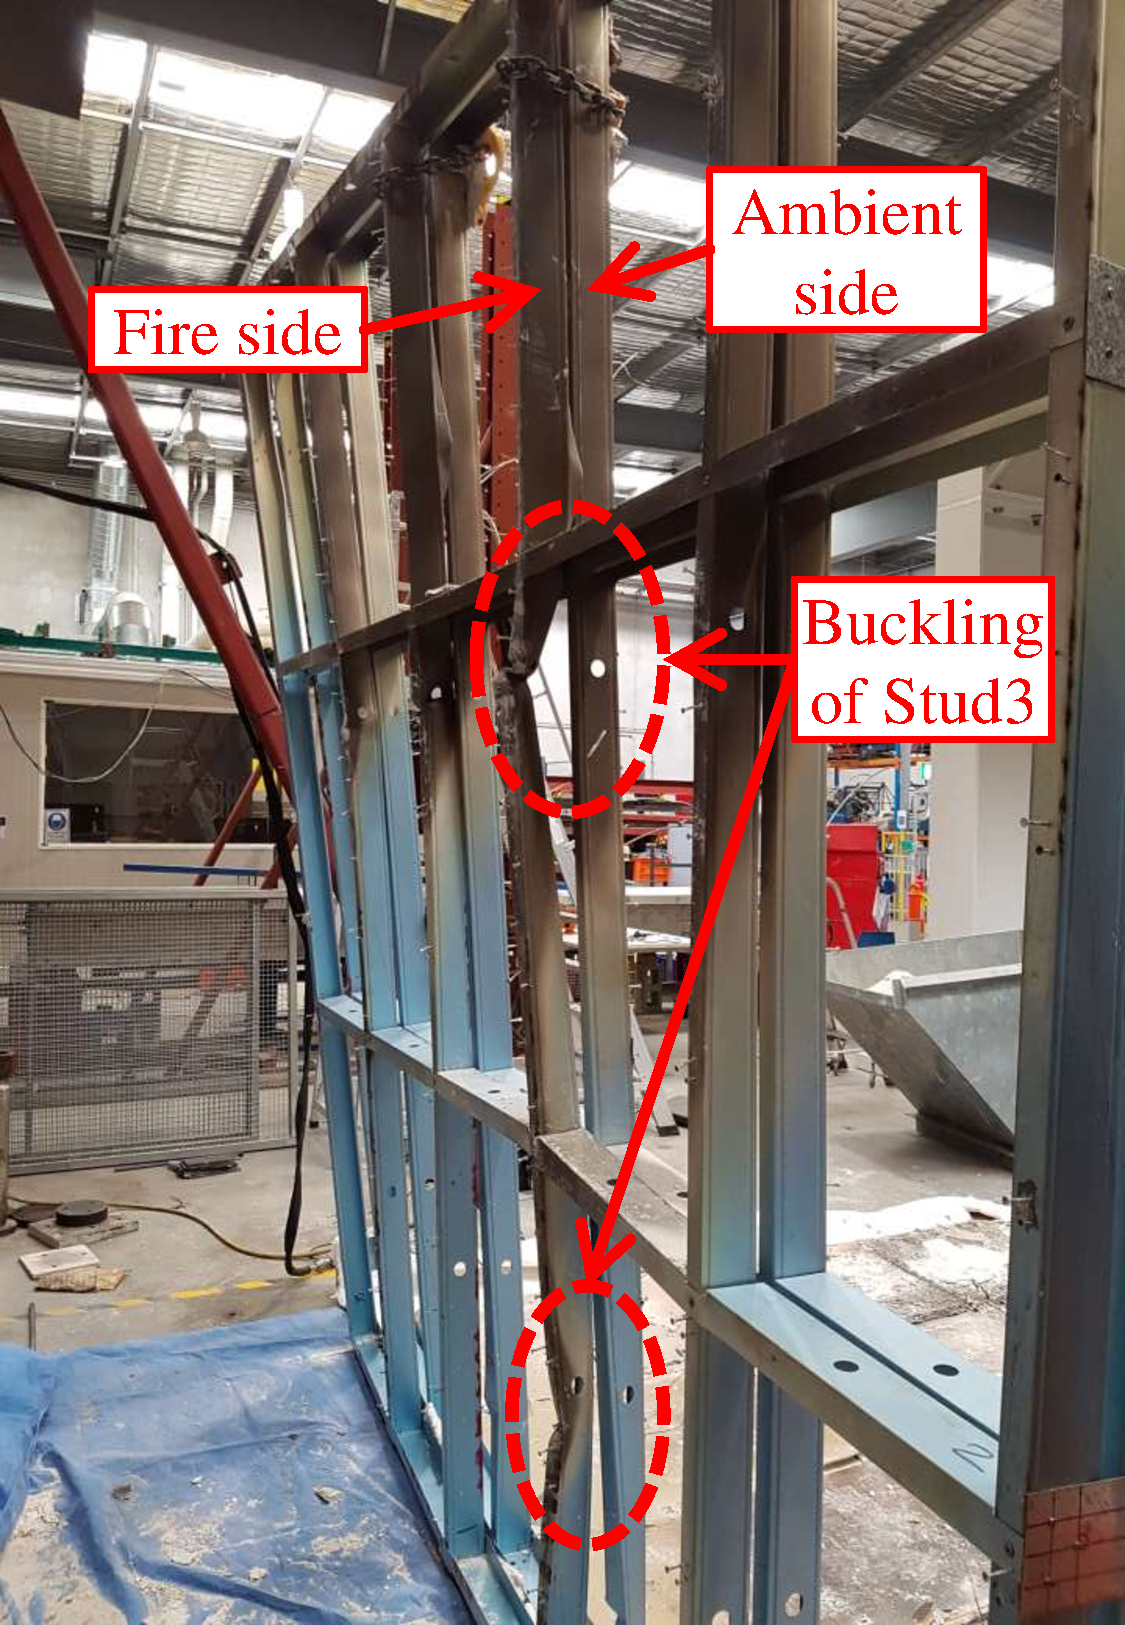
\includegraphics[width=\textwidth]{T1-buckling.pdf}
		\caption{}
		\label{subfig:T1-buckling}
	\end{subfigure}
	   \caption{Failure of Test-T1 wall (a) Fire exposed side (b) Crack on ambient side plasterboard (c) Local compressive failure of Stud3}
	   \label{fig:T1-failure}
\end{figure}

\subsection{Test-T4 Failure Time and Mode, and Observations}